\chapter{Fundamentação teórica}

Este capítulo apresenta os fundamentos teóricos que sustentam o
desenvolvimento da OntoMPO. Inicialmente, são discutidos os conceitos de
observação e transparência e sua relação com a gestão de projetos e com
iniciativas de dados abertos. Em seguida, são apresentados os conceitos de
observatórios e observatórios de projetos, bem como o Modelo para
Observatórios de Projetos (MPO), objeto de formalização desta pesquisa. Por
fim, são discutidos os fundamentos sobre ontologias, incluindo seus
componentes, classificações, a Unified Foundational Ontology (UFO), seus
benefícios e as metodologias empregadas em sua construção, além dos
trabalhos relacionados identificados na literatura.

\section{Observação e transparência}
O uso da observação no contexto do gerenciamento não é um fenômeno recente. Bernstein \cite{bernstein2017making} apresenta uma análise histórica da evolução da observação nas práticas gerenciais, organizando esse processo em diferentes eras. Essas eras são precedidas pelo uso da observação sistemática nos fenômenos naturais e pela consolidação do método científico, que estabeleceram as bases para a incorporação da observação no gerenciamento. Contudo, diferentemente das ciências naturais, nas quais a observação tem como objetivo central a compreensão dos fenômenos, no contexto organizacional ela sempre esteve associada também à intenção de influenciar e, em última instância, controlar comportamentos e processos.

Com o avanço das tecnologias digitais, as organizações passaram a dispor de meios para gerar, processar e transferir grandes volumes de informação a custos marginais reduzidos. Esse cenário, combinado a fenômenos macroeconômicos como a globalização e o aumento da desconfiança nas instituições, deu origem a expectativas públicas sem precedentes em relação à transparência organizacional \cite{heimstadt2017openwashing}. Nesse contexto, as organizações encontram-se inseridas em uma nova era da gestão, caracterizada pela aplicação sistemática da observação, denominada era da transparência \cite{bernstein2017making}.

A transparência pode ser definida como a disponibilidade de informações sobre um determinado ator, possibilitando que outros indivíduos acompanhem ou monitorem seu funcionamento e desempenho \cite{meijer2013understanding}. É importante distinguir, entretanto, se o agente responsável pela divulgação das informações é um indivíduo — associado ou não a uma organização — ou a própria organização \cite{heimstadt2017openwashing}. Quando informações organizacionais se tornam acessíveis a observadores externos por meio de denúncias, a transparência está fortemente relacionada à motivação e ao engajamento do indivíduo envolvido. Já no contexto interno das organizações, a transparência manifesta-se quando decisões deixam de ser pautadas por arbitrariedades individuais e passam a ser estruturadas em programas e critérios de desempenho \cite{meijer2013understanding}.

Do ponto de vista organizacional, a transparência pode ser compreendida como a divulgação sistemática de informações que atendem às necessidades de outros atores. Na teoria da gestão e da organização, esse conceito tem sido tratado como um termo agregador de diferentes construtos, relevantes sobretudo por seus efeitos sobre o desempenho dos indivíduos e das organizações \cite{heimstadt2017openwashing}. Nesse sentido, a transparência pode ser analisada a partir de dimensões como monitoramento, visibilidade dos processos, vigilância e divulgação de informações.

\section{Projetos e transparência}
Um projeto pode ser definido como um esforço temporário empreendido para criar um produto, serviço ou resultado único. O gerenciamento de projetos, por sua vez, corresponde à aplicação de conhecimentos, habilidades, ferramentas e técnicas às atividades do projeto, com o objetivo de atender aos seus requisitos \cite{guide2001project}.

A transparência constitui uma característica recorrente no desenvolvimento de projetos e em seus processos de implementação, embora sua operacionalização varie significativamente entre diferentes metodologias de gerenciamento \cite{betta2018transparency}. Nos modelos clássicos de gerenciamento de projetos, a transparência tende a ser compreendida principalmente como a função de informar as partes interessadas por meio de práticas tradicionais de comunicação, tais como reuniões, comunicados e relatórios formais sobre o andamento do projeto. Abordagens mais recentes, entretanto, elevam a transparência a um nível axiológico, ampliando sua compreensão para além da simples divulgação de informações. Nesses modelos, a transparência passa a envolver o uso de ferramentas e práticas que favorecem a compreensão compartilhada dos processos e procedimentos de gestão, promovendo fluxos bidirecionais de informação e contribuindo para a construção de confiança pessoal e institucional entre os participantes do projeto \cite{betta2018transparency}.

Os projetos desempenham um papel central na promoção da inovação e da mudança organizacional, sendo o principal meio pelo qual organizações implementam estratégias, inovam e obtêm vantagens competitivas \cite{van20147}. Nesse contexto, a transparência pode ser entendida tanto como uma condição quanto como uma ferramenta essencial para o gerenciamento eficaz de projetos \cite{betta2018transparency}. Sua presença não se limita a iniciativas públicas de prestação de contas ou a projetos de software de código aberto, nos quais os artefatos são amplamente acessíveis à comunidade, mas estende-se a diferentes tipos de projetos e contextos organizacionais \cite{trois2017transparency, dabbish2012leveraging}.

Considerando os elementos fundamentais da transparência — monitoramento, visibilidade dos processos, vigilância e divulgação — conforme discutidos por \citeauthor{bernstein2017making}, observa-se que essas práticas se manifestam de forma contínua no cotidiano dos projetos. Isso ocorre por meio de ações como o acompanhamento sistemático do progresso, a disponibilização de informações sobre processos para as equipes envolvidas e a adoção de mecanismos de controle responsáveis, voltados à integridade e ao sucesso das iniciativas. Dessa forma, a transparência consolida-se como um fator relevante para a eficácia, a colaboração e a coordenação em projetos de diferentes naturezas.

\section{Open data}
Dados abertos, também referidos como Informações Abertas do Setor Público (Public Sector Information – PSI), têm recebido atenção crescente nos últimos anos, tanto no meio acadêmico quanto no âmbito governamental \cite{bertot2010using, bertot2012measurement}. Esse interesse tem se refletido na formulação de um amplo conjunto de políticas públicas voltadas à abertura de dados, desenvolvidas em diferentes contextos institucionais e geográficos \cite{civic_commons, huijboom2011open}. Exemplos relevantes incluem iniciativas adotadas por governos como o dos Estados Unidos e da União Europeia, que estabeleceram diretrizes formais para a disponibilização de dados públicos \cite{open_usa, initiative2018communication}.

As políticas de dados abertos desempenham um papel central na promoção da transparência de longo prazo das informações governamentais \cite{bertot2012measurement}. Ao garantir o acesso público a dados produzidos pelo Estado, tais políticas contribuem para o fortalecimento dos direitos dos cidadãos à informação, amplamente reconhecidos como um princípio fundamental das democracias contemporâneas \cite{allen}. Além disso, a abertura de dados possui o potencial de ampliar a participação social, estimular a interação entre governo e sociedade, promover a capacitação dos usuários e favorecer processos de inclusão social \cite{bertot2010using}. Do ponto de vista econômico, iniciativas de dados abertos também são associadas ao estímulo à inovação e ao crescimento econômico, ao possibilitar o desenvolvimento de novos produtos e serviços baseados em dados públicos \cite{borzacchiello2012impact}.

Um estudo conduzido pelo Ministério do Interior e Relações Exteriores do Reino Unido analisou as políticas de transparência adotadas por cinco países — Austrália, Dinamarca, Espanha, Reino Unido e Estados Unidos — com o objetivo de comparar suas abordagens estratégicas em relação aos dados abertos \cite{huijboom2011open}. Os resultados indicam diferenças significativas entre os países analisados. Enquanto os Estados Unidos enfatizam a transparência como meio de ampliar o engajamento público, a Dinamarca destaca o potencial dos dados abertos para o desenvolvimento de novos produtos e serviços. O Reino Unido, por sua vez, ressalta explicitamente o uso de dados abertos como instrumento para o fortalecimento da aplicação da legislação.

De forma geral, essa comparação evidencia a existência de três principais motivações para a publicação de dados governamentais \cite{huijboom2011open}:
\begin{itemize}
    \item ampliar o controle democrático e a participação política;
    \item promover a inovação em serviços e produtos;
    \item fortalecer a aplicação da legislação;
\end{itemize}

No contexto brasileiro, a política de dados abertos é respaldada pela Lei de Acesso à Informação (LAI), que atribui aos órgãos e entidades do poder público a responsabilidade de garantir \cite{L12527}:
\begin{itemize}
    \item a gestão transparente da informação, assegurando amplo acesso e sua divulgação;
    \item a proteção da informação, garantindo sua disponibilidade, autenticidade e integridade;
    \item a proteção de informações sigilosas e pessoais, observando-se sua disponibilidade, autenticidade, integridade e eventuais restrições de acesso;
\end{itemize}

\section{Observatórios}
Não há, na literatura, uma definição única e consensual para o conceito de “observatório”. De modo geral, os estudos existentes associam os observatórios a instrumentos voltados à observação e à promoção da transparência, envolvendo atividades como coleta, consolidação, armazenamento, análise, compartilhamento e divulgação de dados e informações relacionados a um determinado setor ou área do conhecimento \cite{sakata2013construccao, tinati2015building, vieira2021model, keever2017decada}.

Os observatórios podem assumir diferentes naturezas organizacionais e operacionais. Segundo Duarte \cite{duarte}, é possível classificá-los em três tipos principais: (i) unidade organizacional, quando o observatório se configura como um elemento formal da organização, como um departamento, núcleo ou centro responsável por exercer suas funções; (ii) mecanismo ou processo, quando consiste em um dispositivo organizacional por meio do qual um grupo executa as atividades típicas de um observatório; e (iii) instrumento, quando se materializa como uma tecnologia ou ferramenta utilizada para apoiar o cumprimento dessas funções.

De forma geral, o propósito de um observatório é analisar fenômenos específicos e, a partir dessa análise, produzir resultados que contribuam para a construção e a disseminação de conhecimento. A implantação de observatórios pode gerar benefícios significativos para organizações e para a sociedade, tais como o acesso sistematizado ao conhecimento, o apoio à comunicação, cooperação e colaboração entre atores, a melhoria de processos de planejamento e gerenciamento, bem como o suporte ao desenvolvimento de estudos e pesquisas. Além disso, observatórios podem desempenhar um papel relevante no fortalecimento da democracia, ao promover transparência, accountability e aproximação entre governo e sociedade, além de favorecer a inovação e a construção de visões de futuro \cite{vieira2020universal}.

\section{Observatórios de Projetos}
Os observatórios de projetos compartilham os princípios fundamentais dos observatórios em geral, porém distinguem-se por terem como foco a disponibilização sistemática, objetiva e detalhada de informações específicas sobre projetos. Sua principal finalidade é facilitar a compreensão do desempenho, do andamento e dos resultados dos projetos observados, apoiando a tomada de decisão e o acompanhamento por diferentes partes interessadas. Para isso, observatórios de projetos fazem uso de métricas e indicadores que permitem caracterizar aspectos relevantes dos projetos, bem como de mecanismos de representação e interação, como gráficos, tabelas, espaços de interação entre usuários e projetos e análises detalhadas \cite{vieira2020universal}.

Nesse contexto, os observatórios de projetos desempenham um papel central no fortalecimento da transparência no gerenciamento de projetos, ao promover a centralização, a análise e a divulgação estruturada de informações. Atuando como unidades organizacionais, mecanismos ou instrumentos tecnológicos, esses observatórios oferecem canais abertos para o compartilhamento de dados relevantes, proporcionando maior visibilidade sobre os processos e o progresso dos projetos. A disponibilização de métricas, informações processuais e análises consolidadas contribui para a clareza das ações e decisões tomadas ao longo do ciclo de vida dos projetos, favorecendo a comunicação entre os envolvidos e sustentando práticas de prestação de contas. Além disso, observatórios de projetos apoiam a colaboração, o desenvolvimento de estudos e pesquisas e a geração de conhecimento, estabelecendo uma base consistente para inovação e para uma gestão de projetos mais eficiente e confiável \cite{vieira2021model}.

\section{Modelo para Observatórios de Projetos (MPO)}
O Modelo para Observatórios de Projetos (MPO)\cite{vieira2022thesis} constitui uma referência conceitual para a concepção e a análise de observatórios de projetos, ao estabelecer uma definição estruturada dos elementos que os caracterizam e orientam seu funcionamento \cite{vieira2021model}. O modelo busca sistematizar os principais aspectos envolvidos na observação de projetos, oferecendo uma visão abrangente que contempla tanto elementos estruturais quanto operacionais e sociais.

Conforme ilustrado na Figura~\ref{fig:mpo}, o MPO está organizado em três dimensões principais: Estruturas, Processos e Agentes. Cada uma dessas dimensões agrega um conjunto de subdimensões que, por sua vez, compreendem diferentes elementos responsáveis por caracterizar os observatórios de projetos em seus diversos aspectos.

\begin{figure}[!htb]
    \centering
    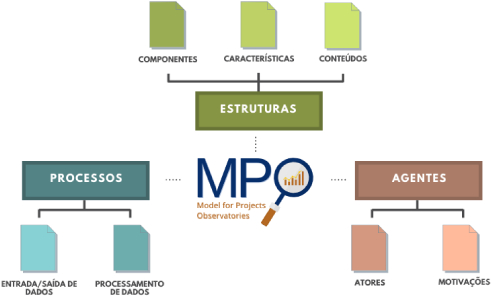
\includegraphics[width=0.5\linewidth]{imagens/mpo.jpg}
    \caption{Representação das dimensões e subdimensões do modelo de Observatório de Projetos. Fonte: \citeauthor{vieira2021model}}
    \label{fig:mpo}
\end{figure}

A dimensão \textbf{Estruturas} reúne os elementos relacionados à configuração estrutural e estática dos observatórios de projetos, contemplando as subdimensões Componentes, Conteúdos e Características. Essa dimensão descreve os aspectos que sustentam o funcionamento do observatório em termos de organização e disponibilização de dados.

\begin{itemize}
    \item \textbf{Componentes:} compreendem os elementos associados à coleta, ao tratamento, ao processamento e à disponibilização dos dados, bem como às estruturas responsáveis por coordenar os relacionamentos entre os atores e sua interação com os projetos e com o próprio observatório;
    \item \textbf{Conteúdos:} referem-se à categorização dos projetos incluídos no observatório e ao registro das observações realizadas pelos participantes humanos sobre os dados e informações disponibilizados;
    \item \textbf{Características:} dizem respeito às propriedades dos dados armazenados no observatório, como sua disponibilidade para os usuários, grau de completude, escopo, natureza estruturada ou não estruturada e as formas de interação dos usuários com esses dados;
\end{itemize}

A dimensão \textbf{Processos} contempla os procedimentos executados no âmbito dos observatórios de projetos, fornecendo uma perspectiva dinâmica de seu funcionamento. Essa dimensão é organizada em subdimensões que descrevem os fluxos e as operações realizadas sobre os dados.

\begin{itemize}
    \item \textbf{Entrada e saída de dados:} abrange as etapas de coleta, armazenamento e compartilhamento de dados, detalhando os fluxos informacionais de forma mais aprofundada do que na dimensão estrutural, ao explicitar como cada etapa do processo é efetivamente realizada;
    \item \textbf{Processamento de dados:} compreende os mecanismos, ferramentas e procedimentos empregados para analisar, compreender, avaliar e interagir com os dados dos projetos de maneira significativa;
\end{itemize}

Por fim, a dimensão \textbf{Agentes} trata dos participantes envolvidos nos observatórios de projetos, considerando tanto sua natureza quanto os fatores que motivam sua interação com o observatório.

\begin{itemize}
    \item \textbf{Atores:} incluem os agentes que participam do observatório, sejam eles indivíduos, grupos organizacionais ou sistemas computacionais;
    \item \textbf{Motivações:} dizem respeito aos fatores que impulsionam os atores a interagir com o observatório, influenciando seu uso, engajamento e contribuição;
\end{itemize}

\section{Ontologias}
O termo ontologia tem origem na Filosofia e refere-se ao estudo da natureza do ser e da realidade última, sendo tradicionalmente compreendido como o conhecimento acerca da essência de tudo o que existe \cite{chaui1995convite}. Trata-se de um campo central da metafísica, explorado ao longo de séculos por diferentes correntes do pensamento filosófico.

Com a incorporação do conceito ao campo da Computação, especialmente a partir dos trabalhos de \citeauthor{neches1991enabling} e \citeauthor{gruber1993translation}, o termo ontologia passou a assumir um significado distinto e operacional. Nesse contexto, ontologias passaram a ser entendidas como especificações formais e explícitas de uma conceitualização compartilhada, capazes de representar conceitos, relações, restrições e regras de um determinado domínio de conhecimento. Essa formalização visa facilitar tanto a compreensão humana quanto o processamento computacional do conhecimento representado.

Em função dessa capacidade de estruturar e explicitar domínios conceituais de maneira rigorosa, as ontologias passaram a desempenhar um papel relevante em diferentes áreas da Computação. Destacam-se, nesse contexto, suas aplicações na Web Semântica \cite{isotani2015ontologias}, na Inteligência Artificial — incluindo abordagens voltadas à explicabilidade dos modelos, como discutido por \citeauthor{confalonieri2023multiple} — e na Engenharia do Conhecimento \cite{gomez2004ontological}. Nas seções seguintes, são apresentados e discutidos os principais componentes e características das ontologias, com ênfase em sua utilização como instrumentos de formalização conceitual.

\subsection{Componentes de uma ontologia}
A construção de uma ontologia envolve a definição de um conjunto de componentes fundamentais responsáveis por explicitar, de forma estruturada e formal, o domínio de conhecimento ao qual ela se aplica. Esses componentes permitem representar conceitos, relações e restrições de maneira precisa, viabilizando tanto a compreensão humana quanto o processamento computacional do conhecimento. Entre os principais componentes de uma ontologia, destacam-se os apresentados por \citeauthor{corcho2005building}  e \citeauthor{gomez2004ontological}.

\begin{itemize}
    \item \textbf{Conceitos (ou classes):} constituem os elementos centrais de uma ontologia, representando categorias ou tipos gerais de entidades em um domínio \cite{isotani2015ontologias}. São caracterizados por seu caráter abstrato e não restrito a instâncias específicas, podendo agrupar diversos outros conceitos relacionados \cite{corcho2005building}. Convencionalmente, as classes são representadas por identificadores iniciados por letra maiúscula, como \textit{Hardware} e \textit{DataManagement}.
    \item \textbf{Relações (ou propriedades):} descrevem a forma como os conceitos de um domínio se associam e interagem entre si. Por meio das relações, é possível expressar dependências, vínculos e interações entre classes. De modo geral, são representadas por identificadores iniciados por letra minúscula, utilizando letras maiúsculas para marcar a concatenação de termos, como em \textit{classifyData}, que pode representar uma relação entre um usuário do observatório e os dados transformados ou indicadores de projetos.
    \item \textbf{Axiomas}: são sentenças lógicas que expressam restrições e regras que devem ser sempre verdadeiras no contexto da ontologia \cite{corcho2005building}. Esses elementos permitem explicitar aspectos do domínio que não podem ser completamente definidos apenas por conceitos e relações, assegurando a coerência semântica do modelo e a consistência das inferências realizadas. Como exemplo, o conceito de \textit{Disponibilidade} pode ser definido pelo axioma $\forall s \in Servico:\ 90 \leq s.Disponibilidade \leq 100$, estabelecendo que a disponibilidade de um serviço deve situar-se entre 90 e 100.
    \item \textbf{Instâncias (ou indivíduos):} representam entidades concretas e específicas pertencentes às classes definidas na ontologia, correspondendo a ocorrências particulares do domínio modelado \cite{corcho2005building}. Por exemplo, \textit{aws} pode ser uma instância da classe \textit{Provider}, enquanto \textit{jose} pode representar uma instância da classe \textit{ObservatoryUser}. Em geral, as instâncias são nomeadas por identificadores iniciados por letra minúscula.
    \item \textbf{Relações (ou propriedades):} descrevem a forma como os conceitos de um domínio se associam e interagem entre si. Por meio das relações, é possível expressar dependências, vínculos e interações entre classes. De modo geral, são representadas por identificadores iniciados por letra minúscula, utilizando letras maiúsculas para marcar a concatenação de termos, como em \textit{classifyData}, que pode representar uma relação entre um usuário do observatório e os dados transformados ou indicadores de projetos.
    \item \textbf{Axiomas}: são sentenças lógicas que expressam restrições e regras que devem ser sempre verdadeiras no contexto da ontologia \cite{corcho2005building}. Esses elementos permitem explicitar aspectos do domínio que não podem ser completamente definidos apenas por conceitos e relações, assegurando a coerência semântica do modelo e a consistência das inferências realizadas. Como exemplo, o conceito de \textit{Disponibilidade} pode ser definido pelo axioma $\forall s \in Servico:\ 90 \leq s.Disponibilidade \leq 100$, estabelecendo que a disponibilidade de um serviço deve situar-se entre 90 e 100.
    \item \textbf{Instâncias (ou indivíduos):} representam entidades concretas e específicas pertencentes às classes definidas na ontologia, correspondendo a ocorrências particulares do domínio modelado \cite{corcho2005building}. Por exemplo, \textit{aws} pode ser uma instância da classe \textit{Provider}, enquanto \textit{jose} pode representar uma instância da classe \textit{ObservatoryUser}. Em geral, as instâncias são nomeadas por identificadores iniciados por letra minúscula.
\end{itemize}

\subsection{Classificação das ontologias}
As ontologias podem receber diferentes classificações de acordo com suas características, sendo comum que uma mesma ontologia se enquadre em mais de uma categoria. As principais classificações encontradas na literatura são \cite{isotani2015ontologias} \cite{gomez2004ontological}:
\begin{itemize}
    \item \textbf{Quanto ao grau de complexidade e formalismo:} Observa-se aqui o grau de formalização e de expressividade lógica empregado nas ontologias. As \textbf{Ontologias Leves} (\textit{Lightweight Ontologies}) adotam um conjunto reduzido de formalismos lógicos e estruturas mais simples, com foco principalmente na organização taxonômica. Por essa razão, apresentam maior facilidade de compreensão e manutenção. Por outro lado, as \textbf{Ontologias Pesadas} (\textit{Heavyweight Ontologies}) incorporam formalismos lógicos mais avançados, como lógica de primeira ordem ou lógica descritiva, além de restrições complexas, axiomas detalhados e suporte a mecanismos de inferência robustos. Essas características permitem capturar nuances semânticas mais profundas, tornando-as particularmente adequadas para domínios complexos e situações em que a precisão conceitual é necessária.
    \item \textbf{Quanto ao nível de generalização}: Aqui, o nível de abstração ou de especificação é o principal fator que orienta a classificação de uma ontologia. As ontologias inicialmente descritas correspondem às \textbf{Ontologias de Topo} (também chamadas de Ontologias Superiores, Ontologias de Top-level ou Upper-Level), que reúnem conceitos altamente abstratos e servem para representar noções fundamentais e universais. Esse tipo de ontologia funciona como base conceitual para a construção de modelos mais específicos \cite{isotani2015ontologias}. A partir desse nível, é possível identificar as \textbf{Ontologias Intermediárias} (também denominadas Core ou Mid-Level), que incluem conceitos de abstração média e estabelecem uma ponte entre as ontologias gerais e as mais especializadas. Por fim, situam-se as \textbf{Ontologias de Aplicação} (ou Domain-Specific), caracterizadas por um elevado grau de detalhamento e voltadas à descrição precisa de domínios específicos.
    \item \textbf{Quanto à finalidade}: \citeauthor{corcho2005building} propõem que as ontologias podem ser classificadas de acordo com seu uso. O primeiro grupo é composto pelas \textbf{Ontologias de Domínio}, cujo propósito central é a reutilização de conceitos. Nesse grupo, incluem-se as Ontologias de Conceito, as Ontologias de Tarefa e as Ontologias Comuns (ou Gerais). O segundo grupo corresponde às \textbf{Ontologias de Comunicação}, voltadas ao compartilhamento de conhecimento entre diferentes agentes ou sistemas. Além desses, há ainda as \textbf{Ontologias de Indexação}, que têm como finalidade apoiar a recuperação eficiente de informações em sistemas de busca, bases de dados e outros ambientes de indexação de conteúdo, e as \textbf{Meta-ontologias}, que desempenham o papel de ontologias voltadas à própria representação do conhecimento.
\end{itemize}

\subsection{A UFO}
A UFO (Unified Foundational Ontology) é uma Ontologia de Topo que estabelece regras, princípios e estereótipos para a definição de conceitos presentes em ontologias de qualquer domínio ou tipo \cite{guizzardi2008grounding}. Ela é composta por um conjunto de sub-ontologias, cada uma voltada a propósitos específicos. Entre as principais, destacam-se:
\begin{itemize}
    \item \textbf{UFO-A}: Trata-se da sub-ontologia dedicada aos \textit{endurants}, elementos que são considerados duradouros, persistentes ou relativamente permanentes, mantendo sua identidade ao longo do tempo \cite{mario2020handling}. Entre as principais classes da UFO-A estão Situation, Role, Phase, Relator, Substantial e Relation. A Figura a seguir apresenta um fragmento ilustrativo da UFO-A.
\end{itemize}
\begin{figure}[!htb]
    \centering
    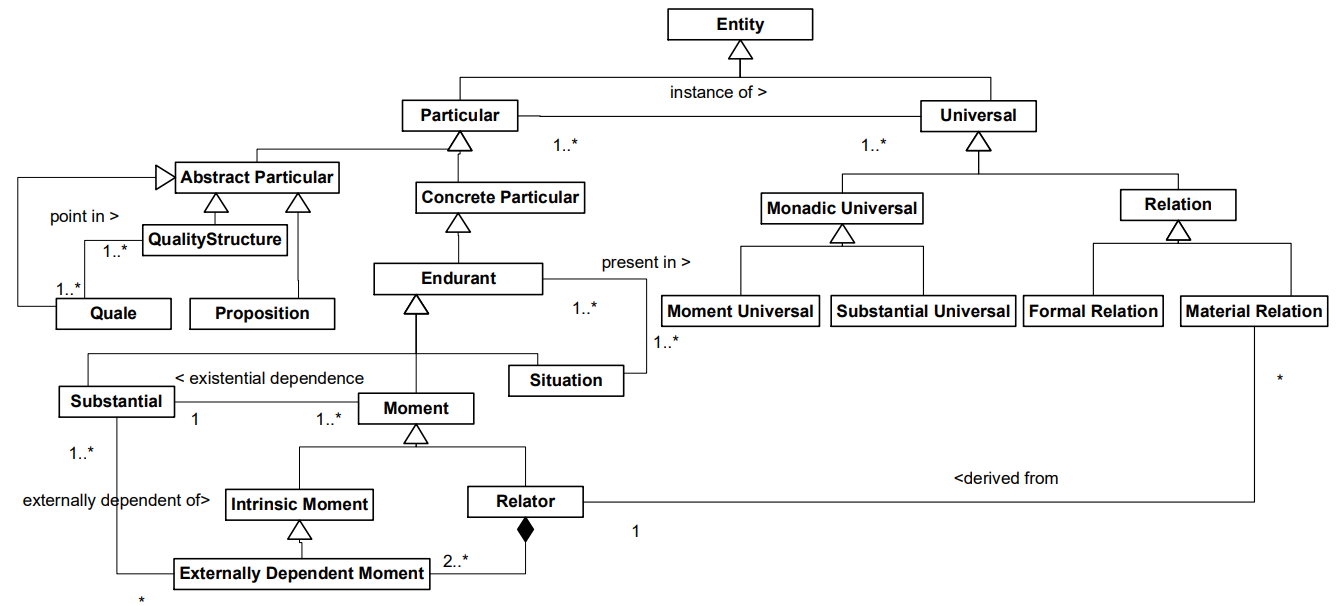
\includegraphics[width=1\linewidth]{imagens/ufo-a.png}
    \caption{Fragmento da ontologia fundamental dos \textit{Endurants} (UFO-A). Fonte: \citeauthor{guizzardi2008grounding}}
    \label{fig:enter-label}
\end{figure}
Na figura apresentada, as setas brancas representam relações de generalização (generalization), isto é, a noção de que dois ou mais conceitos específicos podem ser abstraídos para formar um conceito mais geral. É o caso de \textit{Relator} e \textit{Intrinsic Moment}, que, considerados em conjunto, originam o conceito mais abrangente de \textit{Moment}. O conector sem setas, acompanhado de uma expressão textual, corresponde a uma relação de mediação (\textit{mediation}), indicando que a relação expressa no rótulo estabelece uma mediação entre os conceitos posicionados em suas extremidades. Por fim, o conector em forma de losango preenchido indica uma relação do tipo \textit{ComponentOf}, sinalizando que \textit{Externally Dependent Moment} constitui uma parte integrante de \textit{Relator}.
\begin{itemize}
    \item \textbf{UFO-C}: Trata-se da sub-ontologia das \textit{social entities}, isto é, entidades sociais que incluem papéis, agentes e fenômenos próprios da esfera social. Entre as classes presentes nessa sub-ontologia estão \textit{Agent}, \textit{Goal}, \textit{Normative Description}, \textit{Object} e \textit{Social Roles} \cite{mario2020handling}. A Figura abaixo apresenta um fragmento ilustrativo dessa sub-ontologia.
\end{itemize}
\begin{figure}[!htb]
    \centering
    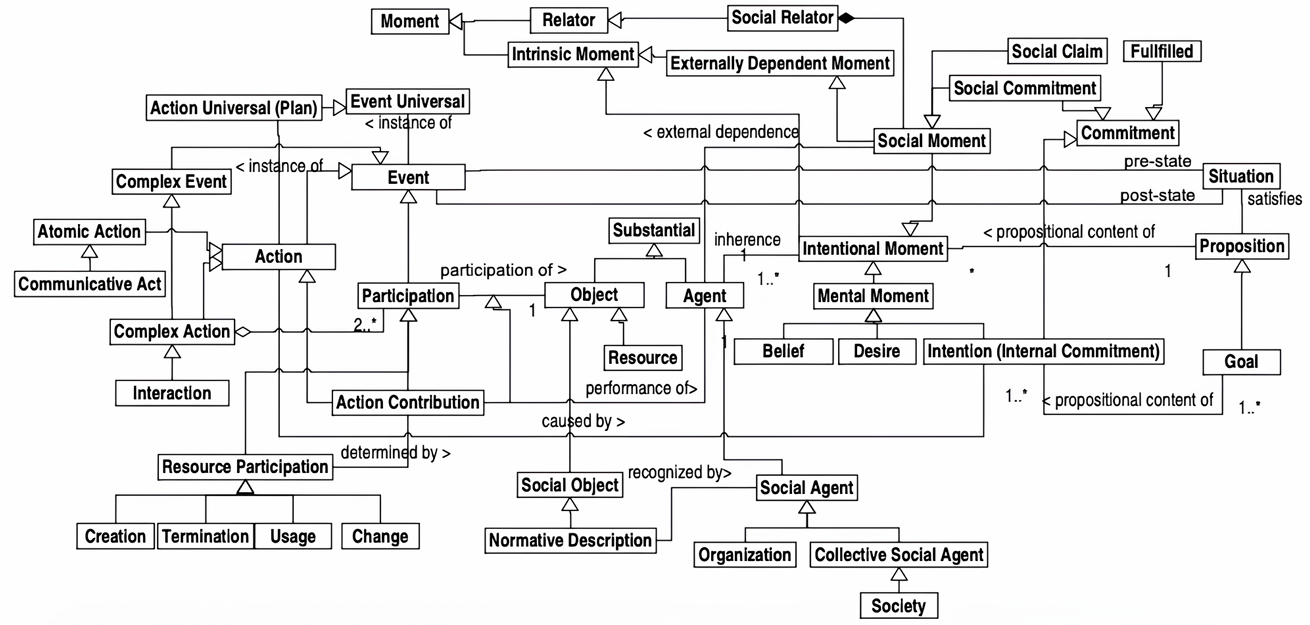
\includegraphics[width=1\linewidth]{imagens/ufo-c.png}
    \caption{Fragmento da ontologia fundamental das \textit{Social Entities} (UFO-C). Fonte: \citeauthor{guizzardi2008grounding}}
    \label{fig:enter-label}
\end{figure}
Todas essas sub-ontologias reúnem conceitos abstratos que são transversais a diferentes contextos, e seu propósito é assegurar a consistência lógica das estruturas conceituais, além de estabelecer um padrão que facilite o reuso e a integração entre ontologias. Dessa forma, é possível e recomendável conectar as classes e características da UFO durante a construção de uma nova ontologia, independentemente da temática ou da classificação adotada.

\subsubsection{OntoUML}
A OntoUML é uma linguagem de modelagem conceitual fundamentada ontologicamente, proposta com o objetivo de apoiar a construção de modelos conceituais semanticamente precisos e com menor grau de ambiguidade. Diferentemente da UML tradicional, que se concentra majoritariamente em aspectos sintáticos e estruturais, a OntoUML é explicitamente baseada na \textit{Unified Foundational Ontology} (UFO), estabelecendo um compromisso ontológico rigoroso entre os elementos do modelo e a realidade que se pretende representar \cite{guizzardi2008grounding, ontouml_readthedocs}.

A motivação central para o uso da OntoUML decorre das limitações observadas em modelos conceituais tradicionais, como os diagramas de classes UML, que frequentemente permitem representações semanticamente inconsistentes ou ambíguas. Essas limitações impactam negativamente a interoperabilidade, o reuso e a evolução dos modelos ao longo do tempo. A OntoUML busca mitigar esses problemas ao impor restrições ontológicas explícitas, especializando os elementos de modelagem a partir de categorias ontológicas bem definidas \cite{ontouml_readthedocs}.

Nesse contexto, a linguagem introduz estereótipos ontológicos como \textit{Kind}, \textit{Subkind}, \textit{Role}, \textit{Phase}, \textit{Relator} e \textit{Collective}, entre outros. Essas categorias derivam diretamente das ontologias fundamentais UFO-A, UFO-B e UFO-C, que tratam, respectivamente, de entidades endurantes, perdurantes e sociais \cite{guizzardi2008grounding}. Cada classe modelada em OntoUML deve ser explicitamente classificada segundo um desses estereótipos, o que impõe regras semânticas rigorosas relacionadas a identidade, rigidez, dependência e relacionalidade.

Por exemplo, um \textit{Kind} representa uma classe que fornece identidade aos seus indivíduos ao longo do tempo, enquanto um \textit{Role} caracteriza uma forma contingente e relacional de participação de uma entidade em um determinado contexto. Essa distinção evita modelagens equivocadas, como a atribuição indevida de identidade a entidades dependentes de contexto, problema recorrente em modelos não fundamentados ontologicamente.

Outro aspecto central da OntoUML é o suporte explícito à diferenciação entre relacionamentos formais e materiais, especialmente por meio do conceito de \textit{Relator}. Esse elemento permite a representação de relações complexas mediadas por entidades sociais ou institucionais, como contratos, acordos ou compromissos, que não podem ser adequadamente expressas por associações binárias simples \cite{ontouml_readthedocs}. Tal capacidade torna a OntoUML particularmente adequada para a modelagem de domínios sociotécnicos, nos quais aspectos organizacionais, normativos e institucionais desempenham papel central.

\subsection{Benefícios}
As ontologias, considerando suas diferentes classificações e propósitos, oferecem um conjunto amplo de benefícios que justificam sua crescente adoção em contextos variados. De maneira geral, esses benefícios estão relacionados à explicitação do conhecimento, à interoperabilidade entre sistemas, ao suporte à inferência automática e à redução de ambiguidades conceituais.

Um dos principais benefícios do uso de ontologias é a explicitação e consolidação de um campo conceitual por meio de um vocabulário padronizado, o que facilita o entendimento compartilhado de um domínio entre diferentes sistemas e usuários. Essa padronização pode ocorrer tanto por meio de representações formais quanto de modelos conceituais diagramáticos, contribuindo para a comunicação clara e precisa do conhecimento. Áreas como a Inteligência Artificial Explicável (XAI) se beneficiam diretamente dessa propriedade, uma vez que a estruturação explícita do conhecimento favorece a interpretabilidade dos modelos \cite{confalonieri2023multiple}.

Outro benefício relevante refere-se à viabilização da interoperabilidade entre sistemas, possibilitando a integração de dados provenientes de fontes heterogêneas. Por meio de ontologias, sistemas distintos podem compreender e compartilhar informações de maneira semântica, reduzindo inconsistências e facilitando a troca de dados em ambientes distribuídos \cite{gonccalves2011using}.

As ontologias também desempenham papel central em mecanismos de busca semântica, promovendo resultados mais relevantes e precisos. Ao incorporar significado às informações, elas permitem uma recuperação de dados mais eficiente, superando limitações de abordagens puramente sintáticas. A Web Semântica constitui um exemplo clássico dessa aplicação, ao utilizar ontologias para estruturar e interligar informações na Web \cite{isotani2015ontologias}.

Além disso, ontologias oferecem suporte à inferência lógica automática, possibilitando a dedução de novas informações a partir de relações, restrições e axiomas definidos no modelo conceitual. Esse aspecto permite enriquecer bases de conhecimento sem a necessidade de inserção manual de todos os fatos, aumentando o poder expressivo e analítico dos sistemas baseados em ontologias \cite{mario2020handling}.

No contexto de sistemas inteligentes, as ontologias contribuem significativamente para a tomada de decisão em domínios complexos, ao permitir inferências fundamentadas em conhecimento formalmente representado. Um exemplo é o uso de ontologias específicas de domínio em tarefas de automação robótica, conforme demonstrado no estudo de \citeauthor{kattepur2018knowledge}, no qual o conhecimento estruturado orienta o comportamento do sistema.

Outro benefício importante é o reuso de conhecimento, especialmente por meio da reutilização de ontologias previamente desenvolvidas como base para novas ontologias de domínio. Essa prática promove a reaplicação de conceitos e relações já consolidados, reduzindo esforço de modelagem e ampliando o alcance dos benefícios associados ao uso de ontologias em diferentes áreas \cite{corcho2005building}.

As ontologias também apresentam maior capacidade de adaptação a mudanças nos requisitos ou na evolução do conhecimento do domínio. Por não constituírem modelos estáticos, elas podem ser ajustadas e estendidas à medida que o domínio se transforma, tanto no âmbito teórico quanto prático \cite{kondylakis2013ontology}.

Por fim, o uso de ontologias contribui para a redução de ambiguidades na representação de conceitos e relações, aumentando a precisão semântica dos modelos. Essa característica tem se mostrado especialmente relevante no contexto de sistemas de inteligência artificial generativa, nos quais a estruturação semântica do conhecimento pode auxiliar na mitigação de alucinações e na produção de respostas mais consistentes \cite{caufield2024structured}.
\section{Trabalhos relacionados}
Foi realizada uma busca sistemática por trabalhos que abordassem de forma integrada os conceitos de observatórios e ontologias \cite{chen2008apply, fox2009ontology, masmoudi2018ontology, yoshiura2018towards}. A análise desses estudos evidenciou que, embora existam iniciativas que utilizam ontologias para representar e organizar conhecimento em diferentes domínios, não foram identificados trabalhos que explorem explicitamente essa integração no contexto específico de observatórios de projetos.

Os estudos encontrados concentram-se, em geral, na aplicação de ontologias como mecanismos de representação formal do conhecimento, com o objetivo de estruturar informações, apoiar processos analíticos ou facilitar a interoperabilidade entre sistemas. Cada uma das ontologias analisadas foi desenvolvida para um domínio particular, refletindo necessidades e características específicas desses contextos.

Dessa forma, observa-se uma lacuna na literatura no que se refere à formalização ontológica de observatórios de projetos, especialmente no que diz respeito à tradução de modelos conceituais existentes em estruturas computacionalmente operacionalizáveis. Este trabalho insere-se nesse contexto ao propor uma ontologia voltada especificamente ao domínio de observatórios de projetos, alinhada ao MPO, contribuindo para o avanço da pesquisa na interseção entre ontologias, transparência e gerenciamento de projetos.

\subsection{\texorpdfstring{\citeauthor{chen2008apply}}{Chen}}
O trabalho de \citeauthor{chen2008apply} propõe um \textit{framework} para apoiar a recuperação e o processamento de imagens no contexto da pesquisa auroral, combinando sistemas multiagentes e ontologias. O objetivo central é facilitar o acesso, a integração e a troca de informações provenientes de múltiplas fontes de dados, permitindo que os pesquisadores concentrem seus esforços na análise científica, sem a necessidade de lidar diretamente com a complexidade dos sistemas de gerenciamento de imagens e dos algoritmos de processamento envolvidos \cite{chen2008apply}.

O \textit{framework} é composto por diferentes tipos de agentes, entre os quais se destacam o Agente Pessoal (\textit{Personal Agent – PA}), responsável por representar o usuário no sistema, e o Agente Corretor (\textit{Broker Agent}), encarregado de identificar e selecionar os agentes de serviço mais adequados para executar as tarefas solicitadas. O PA interpreta as intenções do usuário, decompõe as requisições em subtarefas e coordena a comunicação entre os agentes envolvidos, promovendo a cooperação no ambiente multiagente \cite{chen2008apply}.

Nesse contexto, a ontologia desempenha um papel fundamental como mecanismo de representação e organização do conhecimento do domínio. Sua utilização permite a padronização semântica das informações relacionadas às imagens aurorais, assegurando uma compreensão compartilhada entre agentes e usuários. Além disso, a ontologia é empregada para enriquecer semanticamente os serviços disponibilizados, viabilizando o \textit{matchmaking} semântico entre solicitações dos usuários e capacidades dos serviços oferecidos pelo sistema.

A ontologia também fornece uma estrutura conceitual comum que sustenta a atuação coordenada dos agentes em um ambiente compartilhado, possibilitando interpretações consistentes das informações e favorecendo a interoperabilidade entre diferentes fontes de dados. Adicionalmente, ela apoia a organização e a intercomparação de conjuntos de dados de sensoriamento remoto provenientes de múltiplas origens, contribuindo para a recuperação eficiente de informações relevantes no domínio da pesquisa auroral \cite{chen2008apply}.

\subsection{\texorpdfstring{\citeauthor{fox2009ontology}}{Fox}}
O trabalho de \citeauthor{fox2009ontology} descreve o desenvolvimento do \textit{Virtual Solar-Terrestrial Observatory} (VSTO), uma infraestrutura científica voltada à integração e ao acesso a dados nas áreas de física solar e física solar-terrestre, fundamentada no uso de ontologias. O objetivo central do projeto é lidar com a heterogeneidade e a distribuição dos dados científicos por meio de tecnologias da Web Semântica, promovendo interoperabilidade e acesso unificado a grandes volumes de informação.

Para atender a esses requisitos, foram desenvolvidas ontologias específicas capazes de representar formalmente os conceitos, entidades e relações desses domínios científicos em um formato compreensível por máquinas. Essas ontologias servem como base semântica para a organização e integração dos dados, permitindo que diferentes fontes sejam tratadas de maneira coerente e consistente, independentemente de sua origem ou estrutura.

O desenvolvimento do VSTO foi orientado por casos de uso reais, que guiaram a definição dos requisitos de representação do conhecimento e das funcionalidades de interoperabilidade. A partir disso, o sistema possibilita que cientistas com diferentes níveis de conhecimento técnico acessem, consultem e manipulem os dados como se estivessem em um único ambiente local. Esse nível de abstração é viabilizado pelo uso de mecanismos de raciocínio semântico, que ocultam a complexidade técnica subjacente e ampliam a usabilidade do observatório científico.

\subsection{\texorpdfstring{\citeauthor{masmoudi2018ontology}}{Masmoudi}}
O trabalho de \citeauthor{masmoudi2018ontology} propõe um sistema de monitoramento ambiental fundamentado no uso de ontologias, com o objetivo de promover a interoperabilidade semântica entre dados ambientais oriundos de múltiplas fontes. Os autores destacam que esses dados apresentam elevada heterogeneidade semântica, estrutural e sintática, o que constitui um dos principais desafios para sua integração e análise conjunta.

Para enfrentar esse problema, foi desenvolvida uma ontologia modular baseada na \textit{Basic Formal Ontology} (BFO), organizada em diferentes módulos responsáveis por representar conceitos como desastres naturais, processos ambientais, materiais, sensores e medições. A adoção de uma abordagem modular favorece o reuso, a extensibilidade e a evolução da ontologia, permitindo sua adaptação a distintos cenários de monitoramento ambiental.

A ontologia proposta foi avaliada quanto à coerência, interoperabilidade e completude, por meio de métricas de qualidade e de um estudo de caso. Nesse estudo, demonstrou-se a capacidade do modelo ontológico de gerar conhecimento implícito a partir de dados de precipitação, evidenciando o papel das ontologias não apenas na organização dos dados, mas também no suporte à inferência automática.

Adicionalmente, os autores empregaram regras de inferência para a categorização de diferentes tipos de chuva, concluindo que a ontologia atende aos critérios de qualidade definidos. Como trabalhos futuros, são apontadas a integração automática de dados provenientes de diversas fontes e a aplicação da ontologia em cenários de previsão e mitigação de desastres naturais \cite{masmoudi2018ontology}.

\subsection{\texorpdfstring{\citeauthor{yoshiura2018towards}}{Yoshiura}}
O trabalho de \citeauthor{yoshiura2018towards} propõe um modelo conceitual para observatórios de saúde (\textit{Health Observatories – HOs}), fundamentado no uso de tecnologias da Web Semântica. O objetivo principal é apoiar a formulação de políticas públicas, a gestão da saúde e a pesquisa baseada em evidências, contribuindo para a promoção da saúde e para a melhoria da qualidade de vida da população.

No modelo proposto, os observatórios de saúde são estruturados a partir de componentes funcionais e recursos operacionais. Os componentes funcionais abrangem as entradas, relacionadas às fontes e à gestão dos dados; os processos, voltados à produção de indicadores e inteligência em saúde; e os resultados, responsáveis pela comunicação das informações produzidas. Os recursos operacionais incluem aspectos de governança, equipes analíticas, equipes de tecnologia da informação e o uso de tecnologias de informação e comunicação que sustentam o funcionamento do observatório.

A ontologia desempenha um papel central no modelo conceitual dos HOs, sendo integrada à camada semântica da arquitetura proposta. Essa camada é responsável por organizar e estruturar o conhecimento do domínio da saúde de forma formal e padronizada, possibilitando sua interpretação tanto por agentes humanos quanto por sistemas computacionais. Dessa forma, a ontologia contribui para a interoperabilidade semântica entre diferentes fontes de dados e para o suporte à análise e ao uso das informações no contexto dos observatórios de saúde \cite{yoshiura2018towards}.

\begin{table}[H]
\centering
\caption{Comparação entre os trabalhos relacionados e a proposta desta pesquisa}
\label{tab:comparacao_trabalhos}

\begin{tabularx}{\textwidth}{p{2.5cm} p{2.5cm} X X X}
\hline
\textbf{Trabalho} & \textbf{Domínio} & \textbf{Uso de ontologia} & \textbf{Contexto de observatórios} & \textbf{Relação com observatórios de projetos} \\
\hline
\citeauthor{chen2008apply} \cite{chen2008apply} 
& Pesquisa auroral 
& Representação semântica e suporte a sistemas multiagentes 
& Observatório científico de dados ambientais 
& Não aborda observatórios de projetos \\
\citeauthor{fox2009ontology} \cite{fox2009ontology} 
& Física solar 
& Integração semântica de dados científicos 
& Observatório científico virtual (VSTO) 
& Não aborda observatórios de projetos \\
\citeauthor{masmoudi2018ontology} \cite{masmoudi2018ontology} 
& Monitoramento ambiental 
& Ontologia baseada em BFO para interoperabilidade de dados 
& Não trata explicitamente de observatórios 
& Não aborda observatórios de projetos \\
\citeauthor{yoshiura2018towards} \cite{yoshiura2018towards} 
& Observatórios de saúde 
& Estrutura semântica para organização do conhecimento em saúde 
& Observatórios voltados a políticas públicas de saúde 
& Não trata do domínio de projetos \\
\textbf{Este trabalho}
& Observatórios de projetos 
& Ontologia fundamentada na UFO e modelada em OntoUML 
& Estrutura conceitual baseada no MPO 
& Formalização ontológica do domínio de observatórios de projetos \\
\hline
\end{tabularx}
Fonte: Próprio autor.
\end{table}

